\documentclass[]{article}
\usepackage{amsmath}
\usepackage[margin=1.3cm]{geometry}
\usepackage{amsthm}
\usepackage{listings}
\usepackage{graphicx} %for the fugures
\usepackage{hyperref}
%\usepackage{cleveref} %for the cref command

\title{Practical Lab Numerical Computing Computational Finance \\Bachelor-Worksheet 2}
\author{Lukas Troska, Ilja Kalmykov}
\date{}
\setlength{\parindent}{0pt}

\begin{document}
\maketitle 

The source code can be found at \url{https://github.com/iljaGH/CompFin/}.

\section*{Task 1} Estimation of mean and variance of call-option prices with $K=10,S(0)=10,\mu=0.1,T=2,\Delta t=0.2$ and varying $\sigma$. Larger values of $\sigma$ lead to a bigger mean. This is
due to the price of the call-option
\begin{eqnarray*}
V_{call}\left(S,T\right) & = &\max \lbrace S(T)-K,0 \rbrace
\end{eqnarray*}

always being positive. See task1.cpp for code.
\begin{figure}[!ht]
\centering
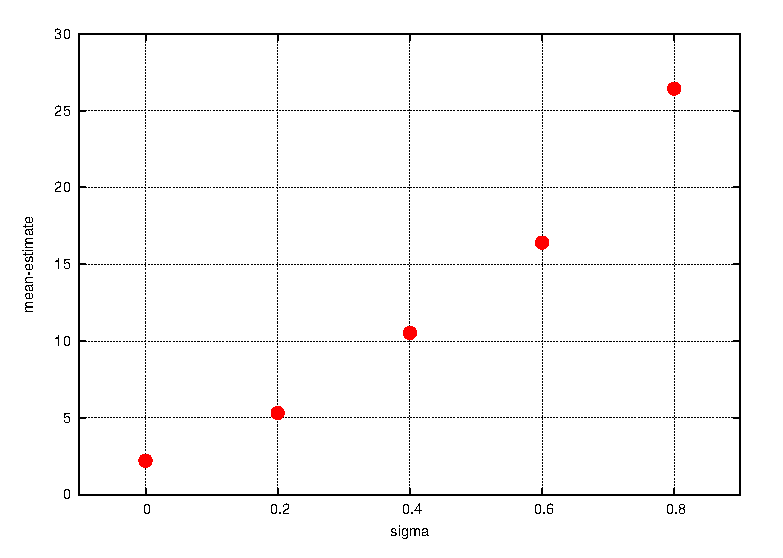
\includegraphics{task1Plot}
\caption{mean estimate for the call-option prices for different values of
$\sigma$.}
\label{fig:Task1}
\end{figure}


\section*{Task 2} Estimation of mean and variance of call-option prices with $K=10,S(0)=10,\mu=0.1,\sigma=0.2,T=2$ and varying $\Delta t$. As we can see in the sample output below, the variance does not depend on $\Delta t$, since the small differences can be caused by the (relatively) small sample size of $N=1000$.
\begin{lstlisting}[caption = estimated $\mu$ and $\sigma$ for
different values of $\Delta t$ and N = 1.0E3, captionpos=b, label=lst:Task2] 
delta t = 0.2 mean = 2.874 variance = 3.811
delta t = 0.4 mean = 2.727 variance = 3.429
delta t = 0.5 mean = 3.001 variance = 3.752
delta t = 1   mean = 2.847 variance = 3.747
delta t = 2   mean = 3.214 variance = 3.885
\end{lstlisting}

\section*{Task 3}
\begin{eqnarray*}
\cfrac{1}{\sqrt{2\pi}}\int_{\chi}^{\infty}K\exp\left(-\cfrac{s^2}{2}\right)ds &
= & \cfrac{1}{\sqrt{2\pi}}\left(\int_{-\infty}^{\infty}K\exp\left(-\cfrac{s^2}{2}\right)ds
- \int_{-\infty}^{\chi}K\exp\left(-\cfrac{s^2}{2}\right)ds \right) \\
& = & K\left(1 - \Phi(\chi)\right) = K \Phi(-\chi)
\end{eqnarray*}

\section*{Task 4}
Approximation of the fair price of a call option with $K=10,S(0)=10,\mu=0.1,\sigma=0.2,T=1,\Delta t=1$. See task4.cpp and for code. 
\begin{figure}[!ht]
\centering
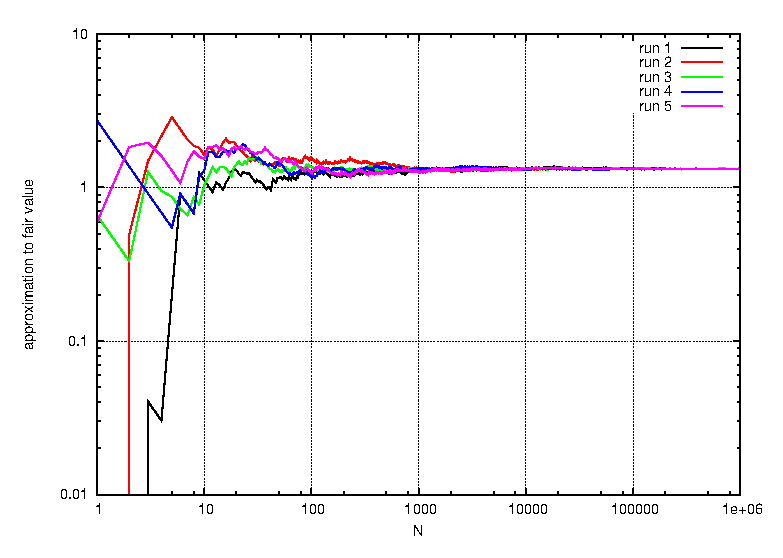
\includegraphics{task4Plot}
\caption{Approximation of $E\left[V_{call}(S_T,0)\right]$.}
\label{fig:Task4a}
\end{figure}
\begin{figure}[!ht]
\centering
\includegraphics{task4Plot_err}
\caption{Convergence plot of approximation above.}
\label{fig:Task4b}
\end{figure}
\clearpage

\section*{Task 5} This formula is just a transformation. We have
\[\Phi(x)=\dfrac{1}{\sqrt{2\pi}}\int_{-\infty}^x
\exp\left({-\dfrac{t^2}{2}}\right)dt\] 
and thus
\[\Phi'(x)=\dfrac{1}{\sqrt{2\pi}}\exp\left({-\dfrac{x^2}{2}}\right)\]

For the derivative of the inverse we have in general, with $y = f(x)$:
\[\left(f^{-1}\right)'(y) = \left(f'\left(f^{-1}(y)\right)\right)^{-1}\]

and thus for the cumulative distribution function we get:
\begin{eqnarray}
\left(\Phi^{-1}\right)'(y) & = &
\left(\Phi'(\Phi^{-1}(y)\right)^{-1} \nonumber\\
\Leftrightarrow \quad \Phi'(\Phi^{-1}(y) & = & \left(\Phi^{-1}(y)\right)^{-1}
\label{equ:deriv}
\end{eqnarray}

Applying the transformation $s = \Phi^{-1}(t)$ and eq. (\ref{equ:deriv}) to 
\[\dfrac{1}{\sqrt{2\pi}}\int_{-\infty}^{\infty}f(s)\exp\left({-\dfrac{s^2}{2}}\right)ds\]
and using integration by substitution gives us:
\begin{eqnarray*}
\dfrac{1}{\sqrt{2\pi}}\int_{-\infty}^{\infty}f(s)\exp\left({-\dfrac{s^2}{2}}\right)ds
& = &
\int_{-\infty}^{\infty}f(s)\underbrace{\dfrac{1}{\sqrt{(2\pi)}}\exp\left({-\dfrac{s^2}{2}}\right)}_{\Phi'(\Phi^{-1})(t)
= \frac{1}{\left(\Phi^{-1}\right)'(t)}}ds \\
& =
&\int_{\Phi^{-1}(-\infty)}^{\Phi^{-1}(\infty)}f(\Phi^{-1}(t))\left(\Phi^{-1}\right)'(t)\cfrac{1}{\left(\Phi^{-1}\right)'(t)}ds
\\
& = &
\int_{0}^{1}f(\Phi^{-1}(t))ds
\end{eqnarray*}

\section*{Task 6} See task6.cpp for code. There is a relationship: We get the
nodes on level $(l+1)$ by taking the nodes on level $l$ and putting a new node
equidistant between two old nodes and also putting a new node equidistantly
between $0$ and the first old node, or $1$ and the last old node respectively.
Nodes positions are:
\begin{eqnarray*}
x_i = \cfrac{1}{N_l+1} = \cfrac{1}{2^l}
\end{eqnarray*}

\section*{Task 7}
See task7.cpp for code. We used GSL for Gauss-Legendre quadrature. The nodes for
the gaussian quadrature are the zeroes of the Legendre polynomials.

\clearpage
\section*{Task 8} See task8.cpp for code. Yes, there is a relationship: on level
$l+1$, we have the nodes from level $l$, and inbetween each "old" node we add a
new node as follows: if on level $l$ we have nodes $x_i,x_{i+1}$ at
\[ \dfrac{1}{2}\left(1-\cos\left(\dfrac{\pi i}{N_l+1}\right)\right)\]
 and
\[\dfrac{1}{2}\left(1-\cos\left(\dfrac{\pi(i+1)}{N_l+1}\right)\right)\]
 respectively, then on level $l+1$ they are node $x_{2i}$ and $x_{2i+2}$ respectively, since
\[\dfrac{i}{N_l+1}=\dfrac{2i}{N_{l+1}+1}\]
 (for $i+1$ analogously). We basically add nodes  $x_{i+0.5}$ for $0\le i \le
 N_l$.

\section*{Task 9}
Integration of $f(x)=1+0.1\cdot\exp(0.5\cdot x)$. See task9.cpp for code.
\begin{figure}[!ht]
\centering
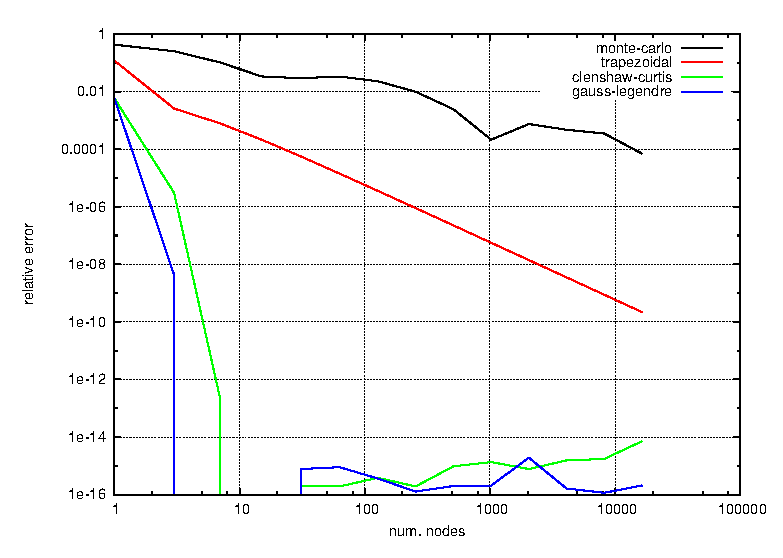
\includegraphics{task9Plot}
\caption{Convergence plot for integration of $f(x)=1+0.1\cdot\exp(0.5\cdot x)$.}
\label{fig:Task9}
\end{figure}
\clearpage

\section*{Task 10}
Integration of $f_{call}\circ \Phi^{-1}=(S(0)\exp((\mu-0.5\cdot\sigma^2)\cdot T+\sigma\sqrt{T}\Phi^{-1}(s))-K)^+$ for a call option with $S(0)=10,\mu=0.1,\sigma=0.2,T=2$ and both $K=0$ and $K=10$. See task10.cpp for implementation.

\begin{figure}[!ht]
\centering
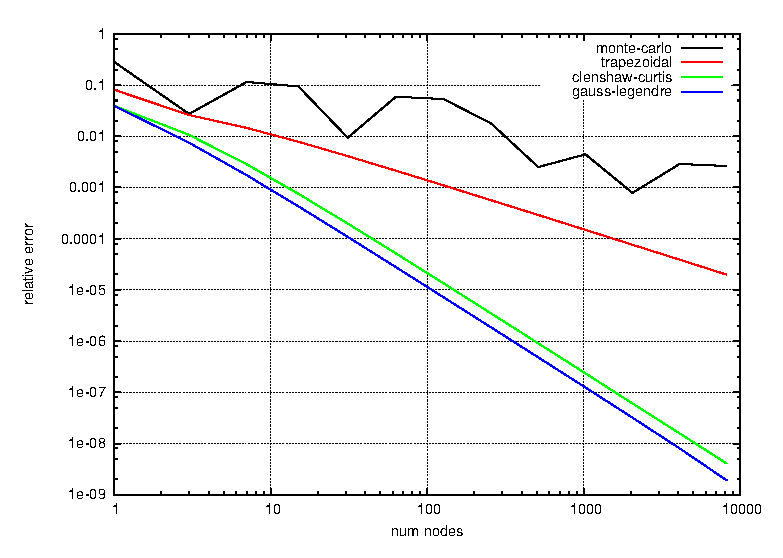
\includegraphics{task10Plot_0}
\caption{Relative error of different integration methods for
$f_{call}\circ \Phi^{-1}$ with $K = 0$.}
\label{fig:Task10_0}
\end{figure}

\begin{figure}[!ht]
\centering
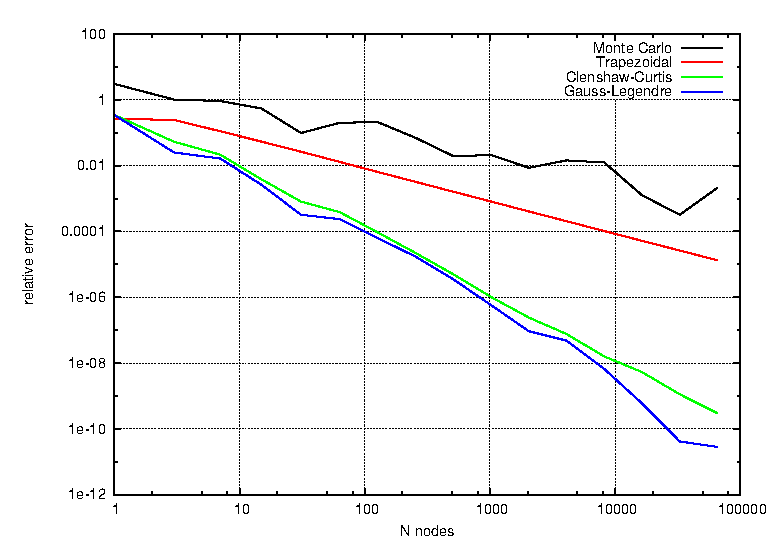
\includegraphics{task10Plot_10}
\caption{Relative error of different integration methods for
$f_{call}\circ \Phi^{-1}$ with $K = 10$.}
\label{fig:Task10_10}
\end{figure}

\end{document}
